
\documentclass[tikz,convert={convertexe={magick.exe}, density=800}]{standalone}
\usepackage{tikzsymbols}
\usepackage{MnSymbol,wasysym}

\begin{document}
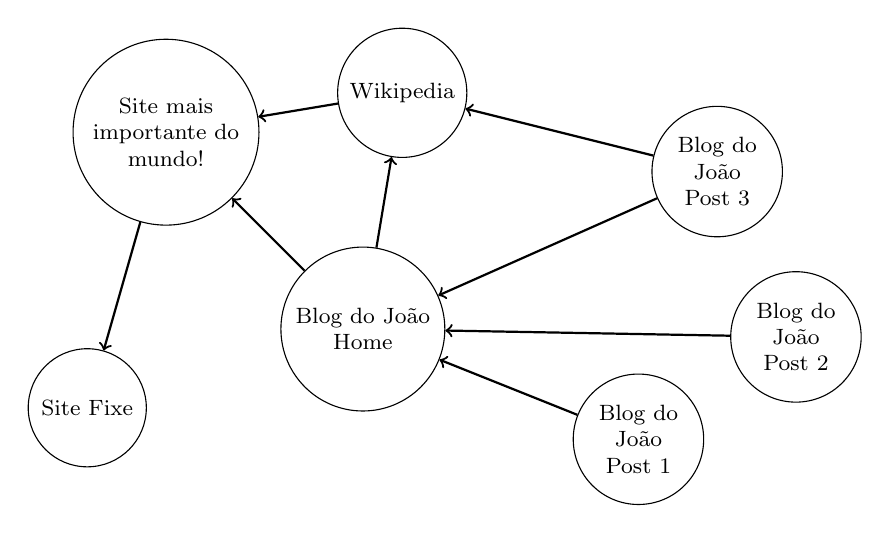
\begin{tikzpicture}[
page/.style={circle, draw, fill=white, minimum size=1.5cm, align=center, font={\footnotesize}},
link/.style={thick,->}
]

    
\node (W) at (-2,0) [page] {Wikipedia};
\node (J1) at (-2.5,-3) [page] {Blog do João\\Home};
\node (I) at (-5,-0.5) [page] {Site mais\\importante do\\mundo!};

\node (J2) at (1, -4.4) [page] {Blog do\\João\\Post 1};
\node (J3) at (3, -3.1) [page] {Blog do\\João\\Post 2};
\node (J4) at (2, -1) [page] {Blog do\\João\\Post 3};

\node (D) at (-6,-4) [page] {Site Fixe};

\draw[link] (J2)--(J1);
\draw[link] (J3)--(J1);
\draw[link] (J4)--(J1);

\draw[link] (J1)--(W);
\draw[link] (J4)--(W);
\draw[link] (I)--(D);

\draw[link] (W)--(I);
\draw[link] (J1)--(I);


\end{tikzpicture}
\end{document}